\documentclass[12pt,a4paper]{report}
\usepackage[utf8]{inputenc}
\usepackage[T1]{fontenc}
\usepackage{lmodern}
\usepackage{graphicx}
\usepackage{xcolor}
\usepackage{hyperref}
\usepackage{tikz}
\usepackage{booktabs}
\usepackage{tcolorbox}
\usepackage{enumitem}
\usepackage{geometry}
\usepackage{fancyhdr}
\usepackage{amsmath}

% Define custom colors
\definecolor{tulipblue}{RGB}{0, 123, 255}
\definecolor{tulipgray}{RGB}{108, 117, 125}
\definecolor{tulipgreen}{RGB}{40, 167, 69}
\definecolor{tulipred}{RGB}{220, 53, 69}
\definecolor{tuliplightgray}{RGB}{248, 249, 250}

% Page setup
\geometry{margin=1in}

% Header and footer
\pagestyle{fancy}
\fancyhf{}
\renewcommand{\headrulewidth}{1pt}
\renewcommand{\footrulewidth}{1pt}
\fancyhead[L]{\textcolor{tulipblue}{Tulip OEE Application}}
\fancyhead[R]{\textcolor{tulipblue}{Training Manual}}
\fancyfoot[C]{\thepage}
\fancyfoot[L]{Moto IE}
\fancyfoot[R]{\today}

% Custom environments
\newenvironment{note}
  {\begin{tcolorbox}[colback=tuliplightgray,colframe=tulipblue,title=Note]}
  {\end{tcolorbox}}

\newenvironment{warning}
  {\begin{tcolorbox}[colback=tuliplightgray,colframe=tulipred,title=Warning]}
  {\end{tcolorbox}}

\newenvironment{tip}
  {\begin{tcolorbox}[colback=tuliplightgray,colframe=tulipgreen,title=Tip]}
  {\end{tcolorbox}}

% Title page
\title{\Huge\textbf{\textcolor{tulipblue}{Tulip OEE Application}\\[0.5cm]\Large Training Manual}}
\author{\Large Moto IE Engineering Team}
\date{\Large \today}

\begin{document}

\maketitle
\thispagestyle{empty}

\newpage
\tableofcontents
\thispagestyle{fancy}

\chapter{Introduction to the Tulip OEE Application}

\section{Purpose and Benefits}

The Tulip OEE (Overall Equipment Effectiveness) Application is a powerful tool designed to help Moto IE engineers monitor, analyze, and improve manufacturing efficiency. This application streamlines data collection, visualization, and reporting processes to provide real-time insights into production performance.

\subsection{Key Benefits}

\begin{itemize}
    \item \textbf{Real-time Monitoring}: Track production metrics in real-time to identify issues as they occur
    \item \textbf{Data-Driven Decision Making}: Base operational decisions on accurate, up-to-date information
    \item \textbf{Customizable Reports}: Generate tailored reports to address specific monitoring needs
    \item \textbf{Performance Visibility}: Access clear visualizations of performance trends across time periods
    \item \textbf{Efficiency Optimization}: Identify bottlenecks and opportunities for improvement
\end{itemize}

\section{OEE Overview}

Overall Equipment Effectiveness (OEE) is a standard measure of manufacturing productivity that combines three essential factors:

\begin{align}
\text{OEE} = \text{Availability} \times \text{Performance} \times \text{Quality}
\end{align}

\begin{figure}[h]
\centering
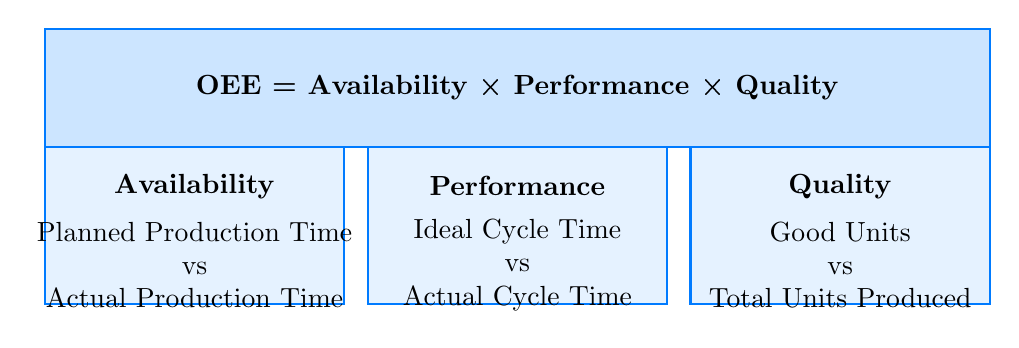
\begin{tikzpicture}
    % OEE Components - Adjusted spacing and sizes
    \draw[fill=tulipblue!20, draw=tulipblue, thick] (0,0) rectangle (12,1.5);
    \node[align=center] at (6,0.75) {\textbf{OEE = Availability × Performance × Quality}};
    
    % Increased vertical spacing between boxes
    % Availability
    \draw[fill=tulipblue!10, draw=tulipblue, thick] (0,-2) rectangle (3.8,-0);
    \node[align=center] at (1.9,-0.5) {\textbf{Availability}};
    \node[align=center] at (1.9,-1.5) {Planned Production Time\\vs\\Actual Production Time};
    
    % Performance - moved horizontally with gap
    \draw[fill=tulipblue!10, draw=tulipblue, thick] (4.1,-2) rectangle (7.9,-0);
    \node[align=center] at (6,-0.5) {\textbf{Performance}};
    \node[align=center] at (6,-1.5) {Ideal Cycle Time\\vs\\Actual Cycle Time};
    
    % Quality - moved horizontally with gap
    \draw[fill=tulipblue!10, draw=tulipblue, thick] (8.2,-2) rectangle (12,-0);
    \node[align=center] at (10.1,-0.5) {\textbf{Quality}};
    \node[align=center] at (10.1,-1.5) {Good Units\\vs\\Total Units Produced};
\end{tikzpicture}
\caption{OEE Components and Calculation}
\end{figure}

\subsection{Understanding OEE Components}

\begin{itemize}
    \item \textbf{Availability} (A): Measures the percentage of scheduled time that the operation is available to operate
    \begin{align}
    \text{Availability} = \frac{\text{Actual Production Time}}{\text{Planned Production Time}} \times 100\%
    \end{align}
    
    \item \textbf{Performance} (P): Measures the speed at which the work center runs as a percentage of its designed speed
    \begin{align}
    \text{Performance} = \frac{\text{Ideal Cycle Time} \times \text{Total Count}}{\text{Operating Time}} \times 100\%
    \end{align}
    
    \item \textbf{Quality} (Q): Measures the good units produced as a percentage of the total units started
    \begin{align}
    \text{Quality} = \frac{\text{Good Count}}{\text{Total Count}} \times 100\%
    \end{align}
\end{itemize}

\begin{tip}
World-class OEE is generally considered to be 85\% or higher. However, the average manufacturing OEE is typically around 60\%.
\end{tip}

\chapter{Getting Started with the Tulip OEE Application}

\section{System Requirements}

Before using the Tulip OEE Application, ensure your system meets the following requirements:

\begin{itemize}
    \item \textbf{Operating System}: Windows 10/11 or macOS 11+
    \item \textbf{Browser}: Google Chrome (latest version), Mozilla Firefox (latest version), or Microsoft Edge (latest version)
    \item \textbf{Internet Connection}: Stable broadband connection (minimum 5 Mbps)
    \item \textbf{Display Resolution}: Minimum 1366 × 768 (recommended: 1920 × 1080)
    \item \textbf{User Permissions}: Access credentials for the Tulip platform
\end{itemize}

\section{Accessing the Application}

To access the Tulip OEE Application:

\begin{enumerate}
    \item Open your web browser
    \item Navigate to \url{https://company-instance.tulip.co/}
    \item Enter your username and password
    \item From the dashboard, select "Applications" from the main menu
    \item Click on "OEE Application" from the list of available applications
\end{enumerate}

\begin{note}
If you don't have login credentials, please contact your system administrator to request access.
\end{note}

\section{User Interface Overview}

The Tulip OEE Application features an intuitive user interface designed for easy navigation and efficient data analysis.

\begin{figure}[h]
\centering
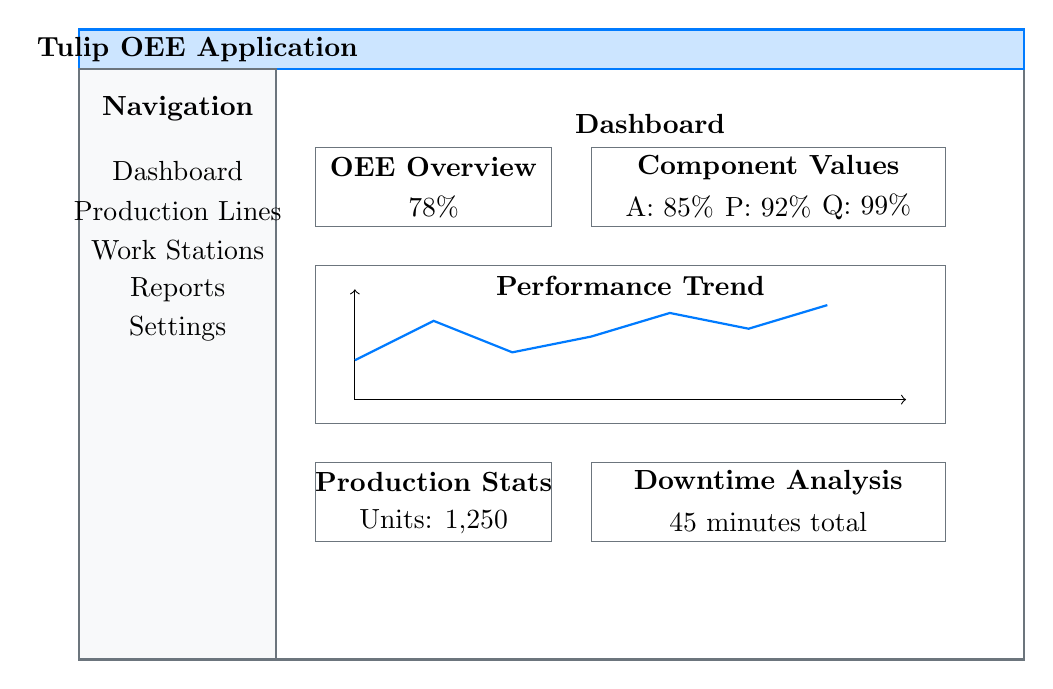
\begin{tikzpicture}
    % Main application window
    \draw[fill=white, draw=tulipgray, thick] (0,0) rectangle (12,8);
    
    % Top navigation bar
    \draw[fill=tulipblue!20, draw=tulipblue, thick] (0,7.5) rectangle (12,8);
    \node[align=left] at (1.5,7.75) {\textbf{Tulip OEE Application}};
    
    % Left sidebar
    \draw[fill=tuliplightgray, draw=tulipgray, thick] (0,0) rectangle (2.5,7.5);
    \node[align=center] at (1.25,7) {\textbf{Navigation}};
    
    % Adjusted vertical spacing for navigation items
    \node[align=left] at (1.25,6.2) {Dashboard};
    \node[align=left] at (1.25,5.7) {Production Lines};
    \node[align=left] at (1.25,5.2) {Work Stations};
    \node[align=left] at (1.25,4.7) {Reports};
    \node[align=left] at (1.25,4.2) {Settings};
    
    % Main content area - moved heading down
    \node[align=center] at (7.25,6.8) {\textbf{Dashboard}};
    
    % OEE Overview widget
    \draw[fill=white, draw=tulipgray] (3,5.5) rectangle (6,6.5);
    \node[align=center] at (4.5,6.25) {\textbf{OEE Overview}};
    \node[align=center] at (4.5,5.75) {78\%};
    
    % Component values
    \draw[fill=white, draw=tulipgray] (6.5,5.5) rectangle (11,6.5);
    \node[align=center] at (8.75,6.25) {\textbf{Component Values}};
    
    % Adjusted horizontal spacing for component values
    \node[align=center] at (7.5,5.75) {A: 85\%};
    \node[align=center] at (8.75,5.75) {P: 92\%};
    \node[align=center] at (10,5.75) {Q: 99\%};
    
    % Performance graph
    \draw[fill=white, draw=tulipgray] (3,3) rectangle (11,5);
    \node[align=center] at (7,4.75) {\textbf{Performance Trend}};
    
    % Draw a simple line graph - adjusted positions
    \draw[->] (3.5,3.3) -- (3.5,4.7);
    \draw[->] (3.5,3.3) -- (10.5,3.3);
    \draw[thick, tulipblue] (3.5,3.8) -- (4.5,4.3) -- (5.5,3.9) -- (6.5,4.1) -- (7.5,4.4) -- (8.5,4.2) -- (9.5,4.5);
    
    % Production stats
    \draw[fill=white, draw=tulipgray] (3,1.5) rectangle (6,2.5);
    \node[align=center] at (4.5,2.25) {\textbf{Production Stats}};
    \node[align=center] at (4.5,1.75) {Units: 1,250};
    
    % Downtime stats
    \draw[fill=white, draw=tulipgray] (6.5,1.5) rectangle (11,2.5);
    \node[align=center] at (8.75,2.25) {\textbf{Downtime Analysis}};
    \node[align=center] at (8.75,1.75) {45 minutes total};
\end{tikzpicture}
\caption{Tulip OEE Application User Interface}
\end{figure}

\subsection{Main Interface Components}

\begin{itemize}
    \item \textbf{Navigation Sidebar}: Access different sections of the application
    \item \textbf{Dashboard}: Overview of key performance metrics
    \item \textbf{Toolbar}: Contains action buttons and filters
    \item \textbf{Data Visualization Area}: Displays charts, graphs, and tables
    \item \textbf{Settings Panel}: Configure application preferences and parameters
\end{itemize}

\chapter{Dashboard and Navigation}

\section{Dashboard Overview}

The dashboard is your central hub for monitoring OEE performance at a glance. It displays key metrics, performance trends, and alerts in a visually intuitive format.

\subsection{Key Dashboard Elements}

\begin{itemize}
    \item \textbf{OEE Summary Cards}: Display current OEE percentage and component values
    \item \textbf{Performance Timeline}: Shows OEE trends over selected time periods
    \item \textbf{Production Statistics}: Provides counts of units produced, rejected, and planned
    \item \textbf{Alerts Panel}: Highlights issues requiring attention
    \item \textbf{Equipment Status}: Visual indicators of machine states
\end{itemize}

\section{Navigating the Application}

\subsection{Using the Navigation Sidebar}

The navigation sidebar provides quick access to different sections of the application:

\begin{itemize}
    \item \textbf{Dashboard}: Return to the main overview screen
    \item \textbf{Production Lines}: View and manage different production lines
    \item \textbf{Work Stations}: Access individual work station data
    \item \textbf{Reports}: Generate and view OEE reports
    \item \textbf{Settings}: Configure application parameters
    \item \textbf{Help}: Access support resources and documentation
\end{itemize}

\subsection{Using Filters and Date Ranges}

The Tulip OEE Application allows you to filter data based on various parameters:

\begin{enumerate}
    \item Click the "Filter" button in the toolbar
    \item Select desired filtering criteria:
    \begin{itemize}
        \item Date range (Today, Yesterday, This Week, Last Week, Custom)
        \item Production line
        \item Work station
        \item Product type
        \item Shift
    \end{itemize}
    \item Click "Apply" to update the displayed data
\end{enumerate}

\begin{tip}
Save frequently used filter combinations by clicking "Save as Preset" in the filter panel. You can quickly apply these presets later.
\end{tip}

\chapter{Customizing OEE Reports}

\section{Creating Custom Reports}

The Tulip OEE Application allows you to create customized reports tailored to your specific requirements.

\subsection{Accessing the Report Builder}

To access the Report Builder:

\begin{enumerate}
    \item Navigate to the "Reports" section using the sidebar
    \item Click on "Create New Report" button
    \item Select "Custom OEE Report" from the template options
\end{enumerate}

\subsection{Defining Report Parameters}

\begin{enumerate}
    \item \textbf{General Settings}:
    \begin{itemize}
        \item Report Name: Enter a descriptive title
        \item Description: Add optional context about the report's purpose
        \item Time Period: Select the date range for analysis
        \item Refresh Rate: Set how often the report updates (if real-time)
    \end{itemize}
    
    \item \textbf{Data Selection}:
    \begin{itemize}
        \item Select Production Lines: Choose specific or all production lines
        \item Select Work Stations: Choose specific or all work stations
        \item Select Products: Filter by product types if needed
        \item Select Shifts: Include specific shifts in analysis
    \end{itemize}
    
    \item \textbf{Metric Selection}:
    \begin{itemize}
        \item OEE Components: Select any combination of Availability, Performance, and Quality
        \item Production Metrics: Units produced, reject rates, downtime, etc.
        \item Custom Calculations: Create custom KPIs based on available data points
    \end{itemize}
\end{enumerate}

\begin{figure}[h]
\centering
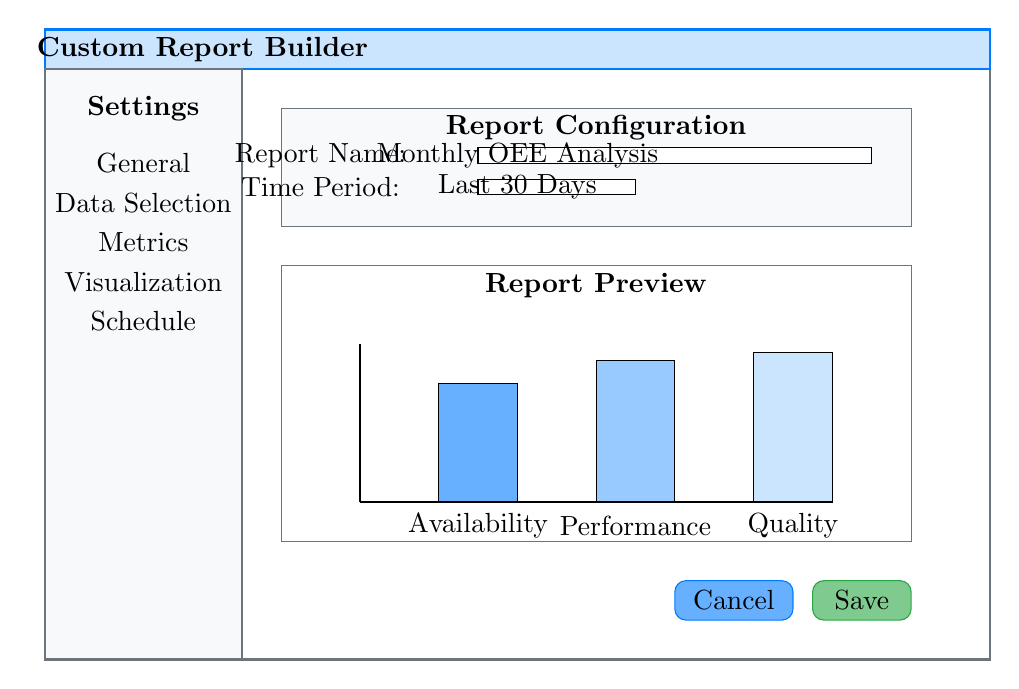
\begin{tikzpicture}
    % Main application window
    \draw[fill=white, draw=tulipgray, thick] (0,0) rectangle (12,8);
    
    % Top navigation bar
    \draw[fill=tulipblue!20, draw=tulipblue, thick] (0,7.5) rectangle (12,8);
    \node[align=left] at (2,7.75) {\textbf{Custom Report Builder}};
    
    % Left sidebar
    \draw[fill=tuliplightgray, draw=tulipgray, thick] (0,0) rectangle (2.5,7.5);
    \node[align=center] at (1.25,7) {\textbf{Settings}};
    
    % Adjusted vertical spacing for settings items
    \node[align=left] at (1.25,6.3) {General};
    \node[align=left] at (1.25,5.8) {Data Selection};
    \node[align=left] at (1.25,5.3) {Metrics};
    \node[align=left] at (1.25,4.8) {Visualization};
    \node[align=left] at (1.25,4.3) {Schedule};
    
    % Main content area - Configuration panel
    \draw[fill=tuliplightgray, draw=tulipgray] (3,5.5) rectangle (11,7);
    \node[align=center] at (7,6.75) {\textbf{Report Configuration}};
    
    % Added more space between form fields
    \node[align=left] at (3.5,6.4) {Report Name:};
    \draw[fill=white] (5.5,6.3) rectangle (10.5,6.5);
    \node[align=left] at (6,6.4) {Monthly OEE Analysis};
    
    \node[align=left] at (3.5,6) {Time Period:};
    \draw[fill=white] (5.5,5.9) rectangle (7.5,6.1);
    \node[align=left] at (6,6) {Last 30 Days};
    
    % Preview area
    \draw[fill=white, draw=tulipgray] (3,1.5) rectangle (11,5);
    \node[align=center] at (7,4.75) {\textbf{Report Preview}};
    
    % Draw a simple bar graph for OEE components - improved spacing
    \draw[thick] (4,2) -- (4,4);
    \draw[thick] (4,2) -- (10,2);
    
    % Bars - adjusted widths and spacing
    \filldraw[fill=tulipblue!60] (5,2) rectangle (6,3.5);
    \filldraw[fill=tulipblue!40] (7,2) rectangle (8,3.8);
    \filldraw[fill=tulipblue!20] (9,2) rectangle (10,3.9);
    
    % Labels - moved down for better spacing
    \node[align=center] at (5.5,1.7) {Availability};
    \node[align=center] at (7.5,1.7) {Performance};
    \node[align=center] at (9.5,1.7) {Quality};
    
    % Buttons - improved spacing
    \draw[fill=tulipblue!60, draw=tulipblue, rounded corners] (8,0.5) rectangle (9.5,1);
    \node[align=center] at (8.75,0.75) {Cancel};
    
    \draw[fill=tulipgreen!60, draw=tulipgreen, rounded corners] (9.75,0.5) rectangle (11,1);
    \node[align=center] at (10.375,0.75) {Save};
\end{tikzpicture}
\caption{Custom Report Builder Interface}
\end{figure}

\section{Visualization Options}

The Tulip OEE Application offers multiple visualization options to present your data effectively.

\subsection{Chart Types}

\begin{itemize}
    \item \textbf{Line Charts}: Ideal for showing trends over time
    \item \textbf{Bar Charts}: Compare values across categories
    \item \textbf{Pie/Donut Charts}: Show proportional distribution
    \item \textbf{Gauge Charts}: Display KPIs against targets
    \item \textbf{Tables}: Present detailed numerical data
    \item \textbf{Heat Maps}: Visualize data intensity across multiple dimensions
\end{itemize}

\subsection{Customizing Visualizations}

\begin{enumerate}
    \item Select the desired chart type from the visualization panel
    \item Configure chart properties:
    \begin{itemize}
        \item Title and description
        \item Axis labels and units
        \item Data series colors
        \item Legends and tooltips
        \item Thresholds and reference lines
    \end{itemize}
    \item Preview the chart in the visualization area
    \item Adjust the size and position of the chart on the report canvas
\end{enumerate}

\begin{tip}
For complex reports, consider using multiple visualization types to present different aspects of your data. For example, use line charts for trends and pie charts for composition analysis.
\end{tip}

\section{Scheduling and Sharing Reports}

\subsection{Setting Up Automated Reports}

To schedule automated report generation and distribution:

\begin{enumerate}
    \item Open the saved report you want to schedule
    \item Click on "Schedule" in the report options menu
    \item Configure the schedule settings:
    \begin{itemize}
        \item Frequency: Daily, Weekly, Monthly, or Custom
        \item Time: When the report should be generated
        \item Start/End dates: Optional duration for the schedule
    \end{itemize}
    \item Set up distribution options:
    \begin{itemize}
        \item Email recipients
        \item File format (PDF, Excel, CSV)
        \item Include message/notes
    \end{itemize}
    \item Click "Save Schedule" to activate
\end{enumerate}

\subsection{Exporting and Sharing Reports}

To manually export and share a report:

\begin{enumerate}
    \item Open the report you want to export
    \item Click on "Export" in the report toolbar
    \item Select the desired export format:
    \begin{itemize}
        \item PDF: Best for presentation and printing
        \item Excel: For further data analysis
        \item CSV: For raw data processing
        \item Image (PNG/JPG): For quick sharing
    \end{itemize}
    \item Choose export options:
    \begin{itemize}
        \item Include raw data: Attach data tables
        \item Page size and orientation
        \item Include filters and parameters
    \end{itemize}
    \item Click "Export" to generate the file
    \item Save locally or share directly via email
\end{enumerate}

\begin{warning}
Be mindful of data sensitivity when sharing reports. Ensure recipients have appropriate authorization to view the information contained in your reports.
\end{warning}

\chapter{Data Analysis and Interpretation}

\section{Understanding OEE Metrics}

Properly interpreting OEE metrics is essential for making data-driven decisions to improve manufacturing efficiency.

\subsection{Interpreting Availability}

Availability measures the percentage of scheduled time that the operation is running. Low availability indicates significant downtime.

\textbf{Common causes of availability losses:}
\begin{itemize}
    \item Equipment failures
    \item Setup and adjustment time
    \item Material shortages
    \item Operator unavailability
    \item Planned maintenance
\end{itemize}

\begin{tcolorbox}[colback=tuliplightgray,colframe=tulipblue,title=Example Analysis]
If your availability is 85\%, it means your operation is running 85\% of the planned production time. For an 8-hour shift, you're losing approximately 1.2 hours to downtime.

\textbf{Action:} Analyze the "Downtime Reasons" report to identify the most frequent or longest causes of downtime. Focus improvement efforts on addressing these specific issues.
\end{tcolorbox}

\subsection{Interpreting Performance}

Performance measures how close your actual production rate is to the ideal (theoretical maximum) rate.

\textbf{Common causes of performance losses:}
\begin{itemize}
    \item Machine wear and reduced speed
    \item Operator inefficiency
    \item Material flow issues
    \item Minor stops and idling
    \item Suboptimal process settings
\end{itemize}

\begin{tcolorbox}[colback=tuliplightgray,colframe=tulipblue,title=Example Analysis]
If your performance is 92\%, your production is running at 92\% of its ideal speed. If your theoretical maximum is 100 units per hour, you're actually producing about 92 units per hour.

\textbf{Action:} Check for machine speed settings, investigate minor stops that may not trigger downtime events, and analyze operator work patterns to identify improvement opportunities.
\end{tcolorbox}

\subsection{Interpreting Quality}

Quality measures the percentage of good units out of total units produced.

\textbf{Common causes of quality losses:}
\begin{itemize}
    \item Process defects
    \item Machine calibration issues
    \item Material defects
    \item Operator errors
    \item Start-up rejects
\end{itemize}

\begin{tcolorbox}[colback=tuliplightgray,colframe=tulipblue,title=Example Analysis]
If your quality rate is 99\%, 1\% of your production is defective. For every 1,000 units, you're producing 10 defective units.

\textbf{Action:} Use the "Quality Defects Pareto" report to identify the most common defect types and their causes, then implement targeted quality improvement initiatives.
\end{tcolorbox}

\section{Using Advanced Analytics}

\subsection{Trend Analysis}

The Tulip OEE Application provides tools for analyzing trends over time:

\begin{enumerate}
    \item Navigate to the "Analytics" section
    \item Select "Trend Analysis" from the options
    \item Choose metrics to analyze (OEE, components, production rate, etc.)
    \item Select time period and grouping (hourly, daily, weekly, monthly)
    \item Apply filters if needed (production lines, products, shifts)
    \item Analyze the resulting trend charts to identify patterns
\end{enumerate}

\begin{figure}[h]
\centering
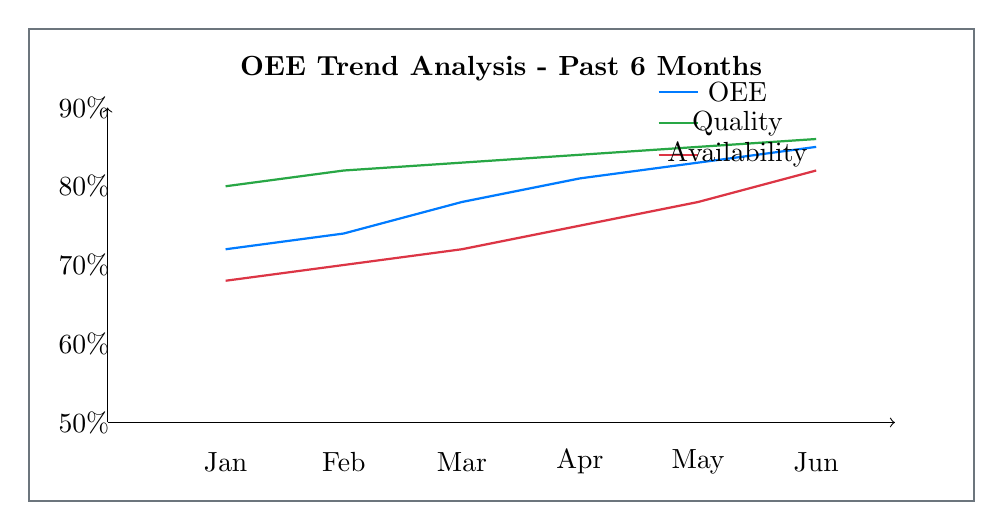
\begin{tikzpicture}
    % Chart area
    \draw[fill=white, draw=tulipgray, thick] (0,0) rectangle (12,6);
    \node[align=center] at (6,5.5) {\textbf{OEE Trend Analysis - Past 6 Months}};
    
    % X and Y axes - adjusted position
    \draw[->] (1,1) -- (1,5);
    \draw[->] (1,1) -- (11,1);
    
    % X-axis labels - improved spacing
    \node[align=center] at (2.5,0.5) {Jan};
    \node[align=center] at (4,0.5) {Feb};
    \node[align=center] at (5.5,0.5) {Mar};
    \node[align=center] at (7,0.5) {Apr};
    \node[align=center] at (8.5,0.5) {May};
    \node[align=center] at (10,0.5) {Jun};
    
    % Y-axis labels - moved left for better spacing
    \node[align=right] at (0.7,1) {50\%};
    \node[align=right] at (0.7,2) {60\%};
    \node[align=right] at (0.7,3) {70\%};
    \node[align=right] at (0.7,4) {80\%};
    \node[align=right] at (0.7,5) {90\%};
    
    % Data lines - kept the same
    \draw[thick, tulipblue] (2.5,3.2) -- (4,3.4) -- (5.5,3.8) -- (7,4.1) -- (8.5,4.3) -- (10,4.5);
    \draw[thick, tulipgreen] (2.5,4.0) -- (4,4.2) -- (5.5,4.3) -- (7,4.4) -- (8.5,4.5) -- (10,4.6);
    \draw[thick, tulipred] (2.5,2.8) -- (4,3.0) -- (5.5,3.2) -- (7,3.5) -- (8.5,3.8) -- (10,4.2);
    
    % Legend - improved spacing and positioning
    \draw[tulipblue, thick] (8,5.2) -- (8.5,5.2);
    \node[align=left] at (9,5.2) {OEE};
    
    \draw[tulipgreen, thick] (8,4.8) -- (8.5,4.8);
    \node[align=left] at (9,4.8) {Quality};
    
    \draw[tulipred, thick] (8,4.4) -- (8.5,4.4);
    \node[align=left] at (9,4.4) {Availability};
\end{tikzpicture}
\caption{OEE Trend Analysis Chart}
\end{figure}

\subsection{Comparative Analysis}

Compare performance across different dimensions:

\begin{enumerate}
    \item Navigate to the "Analytics" section
    \item Select "Comparative Analysis"
    \item Define comparison parameters:
    \begin{itemize}
        \item Metrics to compare
        \item Primary grouping (e.g., Production Lines)
        \item Secondary grouping (e.g., Product Types)
        \item Time period
    \end{itemize}
    \item Analyze results to identify performance variations
\end{enumerate}

\subsection{Root Cause Analysis}

When investigating performance issues:

\begin{enumerate}
    \item Identify the problem area (low OEE, high downtime, quality issues)
    \item Use the "Drill Down" feature to explore detailed data
    \item Apply the "5 Whys" approach using available data
    \item Examine correlation between different factors
    \item Create a Pareto chart of issues to focus on the vital few
\end{enumerate}

\begin{tip}
The "Event Timeline" view can help identify sequences of events that lead to problems, showing how one issue may cascade into others.
\end{tip}

\chapter{Troubleshooting}

\section{Common Issues and Solutions}

This section covers common issues you might encounter when using the Tulip OEE Application and provides solutions.

\subsection{Data Display Issues}

\begin{itemize}
    \item \textbf{Issue}: Charts or metrics not displaying
    \begin{itemize}
        \item \textbf{Solution}: Check your filter settings. Overly restrictive filters may result in no data being available for display.
        \item \textbf{Solution}: Verify the time period selection. Ensure the selected period contains production data.
    \end{itemize}
    
    \item \textbf{Issue}: Unexpected or inaccurate OEE values
    \begin{itemize}
        \item \textbf{Solution}: Check input data quality. Verify that availability, performance, and quality data are being correctly captured.
        \item \textbf{Solution}: Review calculation settings. Ensure the correct ideal cycle times and planned production times are configured.
    \end{itemize}
    
    \item \textbf{Issue}: Slow loading times
    \begin{itemize}
        \item \textbf{Solution}: Reduce the date range or amount of data being processed.
        \item \textbf{Solution}: Check your internet connection speed and stability.
        \item \textbf{Solution}: Close unused browser tabs to free up system resources.
    \end{itemize}
\end{itemize}

\subsection{Access and Login Issues}

\begin{itemize}
    \item \textbf{Issue}: Unable to log in
    \begin{itemize}
        \item \textbf{Solution}: Verify your username and password.
        \item \textbf{Solution}: Check if Caps Lock is enabled.
        \item \textbf{Solution}: Clear browser cache and cookies, then try again.
        \item \textbf{Solution}: Contact your system administrator to verify your account status.
    \end{itemize}
    
    \item \textbf{Issue}: Missing features or limited access
    \begin{itemize}
        \item \textbf{Solution}: Confirm your user role and permissions with your administrator.
        \item \textbf{Solution}: Request additional access rights if needed for your role.
    \end{itemize}
\end{itemize}

\section{Error Messages and Meanings}

\begin{table}[h]
\centering
\begin{tabular}{p{4cm}p{3cm}p{5cm}}
\toprule
\textbf{Error Message} & \textbf{Error Code} & \textbf{Meaning and Solution} \\
\midrule
No data available & ERR-101 & No data exists for the selected filters. Try broadening your search criteria or checking data inputs. \\
\midrule
Connection error & ERR-201 & Unable to connect to the Tulip server. Check your internet connection and try again. \\
\midrule
Authentication failed & ERR-301 & Your login credentials could not be verified. Verify your username and password or contact support. \\
\midrule
Calculation error & ERR-401 & Problem calculating metrics. Check for missing input data or configuration issues. \\
\midrule
Report generation failed & ERR-501 & Unable to generate the requested report. Check report parameters and try again. \\
\midrule
Data sync error & ERR-601 & Problem synchronizing data with production systems. Contact your administrator. \\
\bottomrule
\end{tabular}
\caption{Common Error Messages and Their Solutions}
\end{table}

\section{Getting Help}

If you encounter issues not covered in this section:

\begin{enumerate}
    \item Check the in-app help by clicking the "Help" icon in the navigation bar
    \item Access the knowledge base at \url{https://support.tulip.co/knowledge}
    \item Contact your internal Tulip administrator
    \item Submit a support ticket through the "Support" menu in the application
    \item For urgent issues, contact the support hotline at (555) 123-4567
\end{enumerate}

\begin{note}
When contacting support, include details such as error messages, steps to reproduce the issue, and screenshots if possible. This helps resolve your issue more quickly.
\end{note}

\end{document}